
\documentclass{standalone}
\usepackage{tikz}
\usetikzlibrary{arrows.meta, positioning}

\usepackage{amssymb} 
\usetikzlibrary{shapes.geometric}
\newcommand\px{0}
\begin{document}
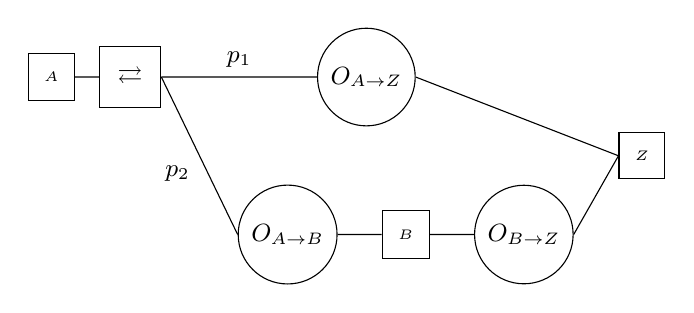
\begin{tikzpicture}[square/.style={regular polygon,regular polygon sides=4}]

    % Probability 
    \node at (\px, 1) [square, draw] (s) {\tiny $A$}; 
    \node at (\px + 1, 1) [square, draw] (probab) {\small $\rightleftarrows$};
    \node at (\px + 4, 1) [circle, draw] (o3) {\small $O_{A \rightarrow Z}$};
    \node at (\px + 3, -1) [circle, draw] (o4) {\small $O_{A \rightarrow B}$};
    \node at (\px + 7.5, 0) [square, draw] (e) {\tiny $Z$};
    \node at (\px + 4.5, -1) [square, draw] (b) {\tiny $B$};
    \node at (\px +6, -1) [circle, draw] (o5) {\small $O_{B \rightarrow Z}$};
    \draw (s.east) -- (probab.west);
    \draw (probab.east) -- (o3.west) node[midway, above] {\small $p_1$};
    \draw (probab.east) -- (o4.west) node[midway, below left] {\small $p_2$};
    \draw (o3.east) -- (e.west);
    \draw (o4.east) -- (b.west);
    \draw (b.east) -- (o5.west);
    \draw (o5.east) -- (e.west);
\end{tikzpicture}
\end{document}
